Initially, an approach similar to that used by Kominami et al., which uses a Hough transform to detect lines in an 
image corresponding to the edges of a perch, then calculates a depth profile perpendicular to those two edges to identify 
the shape and position of the object \cite{kominami_detection_2023}, was tested. However, this approach presented two primary challenges
for this thesis:
\begin{itemize}
    \item When detecting less straight and smooth shapes, such as branches, the Hough transform struggled to detect 
        two opposite edges of the perch due to the uneven edges that such a perch has. 
    \item The method of computing a depth profile between the two edges struggled with the relatively low-quality 
        depth data produced by Raspberry Pi cameras and \texttt{OpenCV}'s stereo block matcher; the clean and sharp
        edges that Kominami et al. used to detect object boundaries and shape are not present, instead this depth data
        contains many artifacts and inaccuracies near object boundaries. This issue is highlighted in Fig. \ref{fig:detect-profile-proto}.
\end{itemize}


\begin{figure}[H]
    \centering
    \begin{subfigure}[b]{\textwidth}
        \begin{subfigure}[b]{0.33\textwidth}
            \centering
            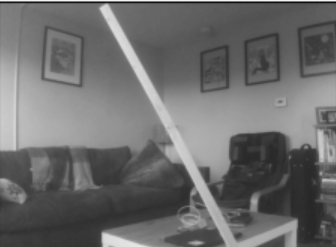
\includegraphics[width=\textwidth]{appendices/detect-proto-img.png}
            \caption{Left camera image of a rectangular test perch.}
            \label{fig:detect-profile-proto:img}
        \end{subfigure}
        \hfill
        \begin{subfigure}[b]{0.33\textwidth}
            \centering
            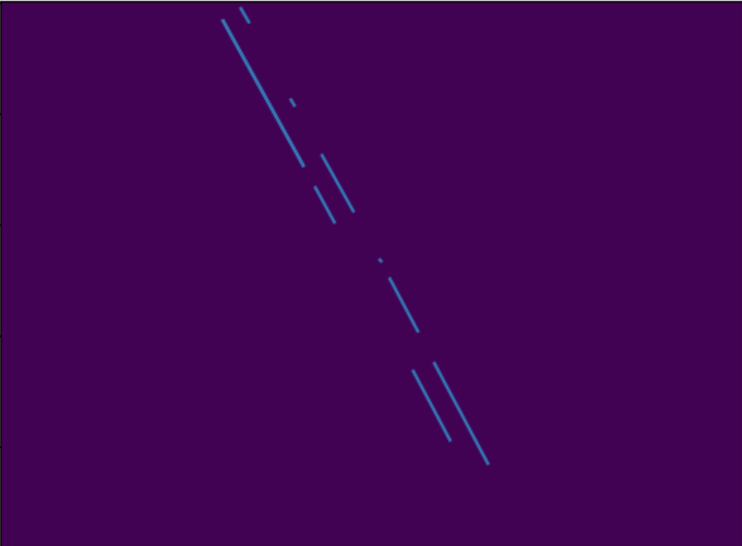
\includegraphics[width=\textwidth]{appendices/detect-proto-lines.png}
            \caption{Image showing the parallel line segments detected in \ref{fig:detect-profile-proto:img}.}
            \label{fig:detect-profile-proto:lines}
        \end{subfigure}
        \hfill
        \begin{subfigure}[b]{0.33\textwidth}
            \centering
            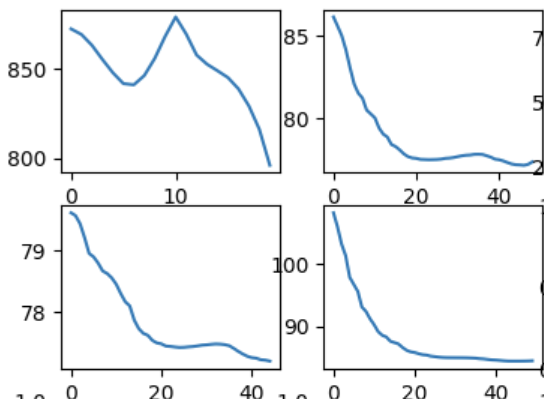
\includegraphics[width=\textwidth]{appendices/detect-proto-depth.png}
            \caption{Select depth profiles between 4 pairs of parallel line segments in \ref{fig:detect-profile-proto:lines}.
            The units of the vertical axes are mm, and the horizontal axes are pixels.}
            \label{fig:detect-profile-proto:depth}
        \end{subfigure}
    \end{subfigure}
    \caption{Test images for a prototype detection method inspired by Kominami et al. \cite{kominami_detection_2023}. 
    \ref{fig:detect-profile-proto:lines} shows multiple pairs of parallel lines that were detected by a Hough transform,
    and \ref{fig:detect-profile-proto:depth} shows the depth profiles between a selection of 4 of these pairs. The feature 
    to note in \ref{fig:detect-profile-proto:depth} is the lack of well-defined edges or a clear level showing the location 
    of the perch, which is the reason this prototype method was not explored further.}
    \label{fig:detect-profile-proto}
\end{figure}


Additionally, the use of a small 8x8 lidar sensor (ST VL53L8CX) to improve confidence of the depth data and verify perch locations was 
explored. The intent was to use this sensor to check the likelihood that a perch detected in the stereo point cloud truly exists,
and remove false detections that are produced by noisy background pixels. This sensor was abandoned because its data quality degrades 
when exposed to sunlight; this makes it unviable for this design since the target application is outdoor use. 